\documentclass[12pt, letterpaper]{article}

% ---------- Paquetes ----------
\usepackage[utf8]{inputenc}
\usepackage[T1]{fontenc}
\usepackage[spanish]{babel}
\usepackage{geometry}
\usepackage{setspace}
\usepackage{graphicx}
\usepackage{float}
\usepackage{hyperref}
\usepackage{fancyhdr}
\usepackage{titlesec}
\usepackage{listings}
\usepackage{xcolor}
\usepackage{caption}
\usepackage{booktabs}
\usepackage{cite}
\usepackage{times}

% ---------- Geometría APA ----------
\geometry{
  letterpaper,
  left=2.54cm,
  right=2.54cm,
  top=2.54cm,
  bottom=2.54cm
}

% ---------- Interlineado doble ----------
\doublespacing

% ---------- Sangría APA (0.5 in = 1.27 cm) ----------
\setlength{\parindent}{1.27cm}

% ---------- Estilo de página ----------
\pagestyle{fancy}
\fancyhf{}
\rhead{\thepage}
\lhead{ACTIVIDAD \#2 -- OWASP JUICE SHOP}
\renewcommand{\headrulewidth}{0pt}

% ---------- Estilo de código ----------
\lstset{
  backgroundcolor=\color{gray!10},
  basicstyle=\ttfamily\footnotesize,
  breaklines=true,
  frame=single,
  rulecolor=\color{gray!40},
  keywordstyle=\color{blue},
  commentstyle=\color{green!50!black},
  stringstyle=\color{red!70!black},
  showstringspaces=false,
  tabsize=2,
  captionpos=b
}

% ---------- Secciones sin numeración automática estilo APA ----------
\titleformat{\section}{\normalfont\large\bfseries\centering}{}{0em}{}
\titleformat{\subsection}{\normalfont\normalsize\bfseries}{}{0em}{}
\titleformat{\subsubsection}{\normalfont\normalsize\bfseries\itshape}{}{0em}{}

% ==========================================================
\begin{document}

% ---------- Portada ----------
\begin{titlepage}
  \centering
  \vspace*{2cm}

  {\large Universidad Tecnológica de Pereira\\
  Facultad de Ingenierías\\
  Especialización en Tecnologías de la Información y las Comunicaciones\\[0.5em]
  Ciberseguridad}

  \vspace{3cm}

  {\LARGE \textbf{Actividad \#2 -- OWASP Juice Shop:\\
  Explotación de Vulnerabilidades Web en Entornos Controlados}}

  \vspace{3cm}

  {\large Daniel Toro Soto}

  \vfill

  {\large Pereira, Colombia\\
  Mayo de 2026}
\end{titlepage}

% ---------- Tabla de contenidos ----------
\tableofcontents
\newpage

% ==========================================================
\section{Introducción}

La seguridad de las aplicaciones web es uno de los pilares fundamentales de la ciberseguridad moderna. Las organizaciones que desarrollan o mantienen aplicaciones accesibles a través de internet están expuestas a una amplia variedad de ataques que buscan comprometer datos, sesiones de usuario y la integridad de los sistemas subyacentes. En este contexto, el proyecto OWASP (\textit{Open Web Application Security Project}) publica periódicamente el \textit{OWASP Top 10}, una clasificación de las vulnerabilidades de seguridad web más críticas y frecuentes.

En el marco de esta actividad académica, se exploran tres categorías del OWASP Top 10 (2021) mediante la explotación controlada de OWASP Juice Shop, una aplicación web deliberadamente vulnerable diseñada para el entrenamiento en seguridad ofensiva. Las vulnerabilidades abordadas corresponden a las categorías A03 (Inyección), A02 (Fallos Criptográficos / Exposición de Datos Sensibles) y A01 (Control de Acceso Roto).

Todas las pruebas se realizaron en un entorno aislado de red (modo Solo Anfitrión) sobre una Mac Mini M4, utilizando UTM como hipervisor para gestionar las máquinas virtuales Kali Linux (atacante) y Ubuntu 22.04 con Juice Shop (víctima).

% ==========================================================
\section{Configuración del Entorno}

\subsection{Descripción del entorno}

El entorno de laboratorio está compuesto por dos máquinas virtuales ejecutadas en UTM sobre una Mac Mini con procesador Apple M4. Ambas máquinas fueron configuradas con una única interfaz de red en modo Solo Anfitrión (\textit{Host-Only}), lo que garantiza el aislamiento total del tráfico respecto a redes externas.

\begin{table}[H]
  \centering
  \caption{\textit{Configuración de las máquinas virtuales}}
  \begin{tabular}{@{}llll@{}}
    \toprule
    \textbf{Máquina} & \textbf{Rol} & \textbf{SO} & \textbf{Dirección IP} \\
    \midrule
    Kali Linux        & Atacante     & Kali Linux 2024 & 192.168.40.3 \\
    Ubuntu + Juice Shop & Víctima    & Ubuntu 22.04    & 192.168.40.11:3000 \\
    \bottomrule
  \end{tabular}
\end{table}

\subsection{Herramientas del entorno}

\begin{itemize}
  \item \textbf{UTM}: Hipervisor para macOS/Apple Silicon que permite ejecutar máquinas virtuales x86\_64 mediante emulación QEMU.
  \item \textbf{Kali Linux}: Distribución GNU/Linux orientada a pruebas de penetración, que incluye de forma nativa herramientas como Firefox, Burp Suite, curl y sqlmap.
  \item \textbf{OWASP Juice Shop}: Aplicación web Node.js deliberadamente vulnerable, diseñada por OWASP para el entrenamiento en seguridad ofensiva. Corre sobre Express y utiliza una base de datos SQLite.
\end{itemize}

\begin{figure}[H]
  \centering
  
\includegraphics[width=0.85\textwidth]{../../img/environment/utm.png}
  \caption{\textit{Vista del hipervisor UTM con las máquinas virtuales activas.}}
\end{figure}

\begin{figure}[H]
  \centering
  
\includegraphics[width=0.85\textwidth]{../../img/environment/kali.png}
  \caption{\textit{Máquina virtual Kali Linux (atacante) en ejecución.}}
\end{figure}

\begin{figure}[H]
  \centering
  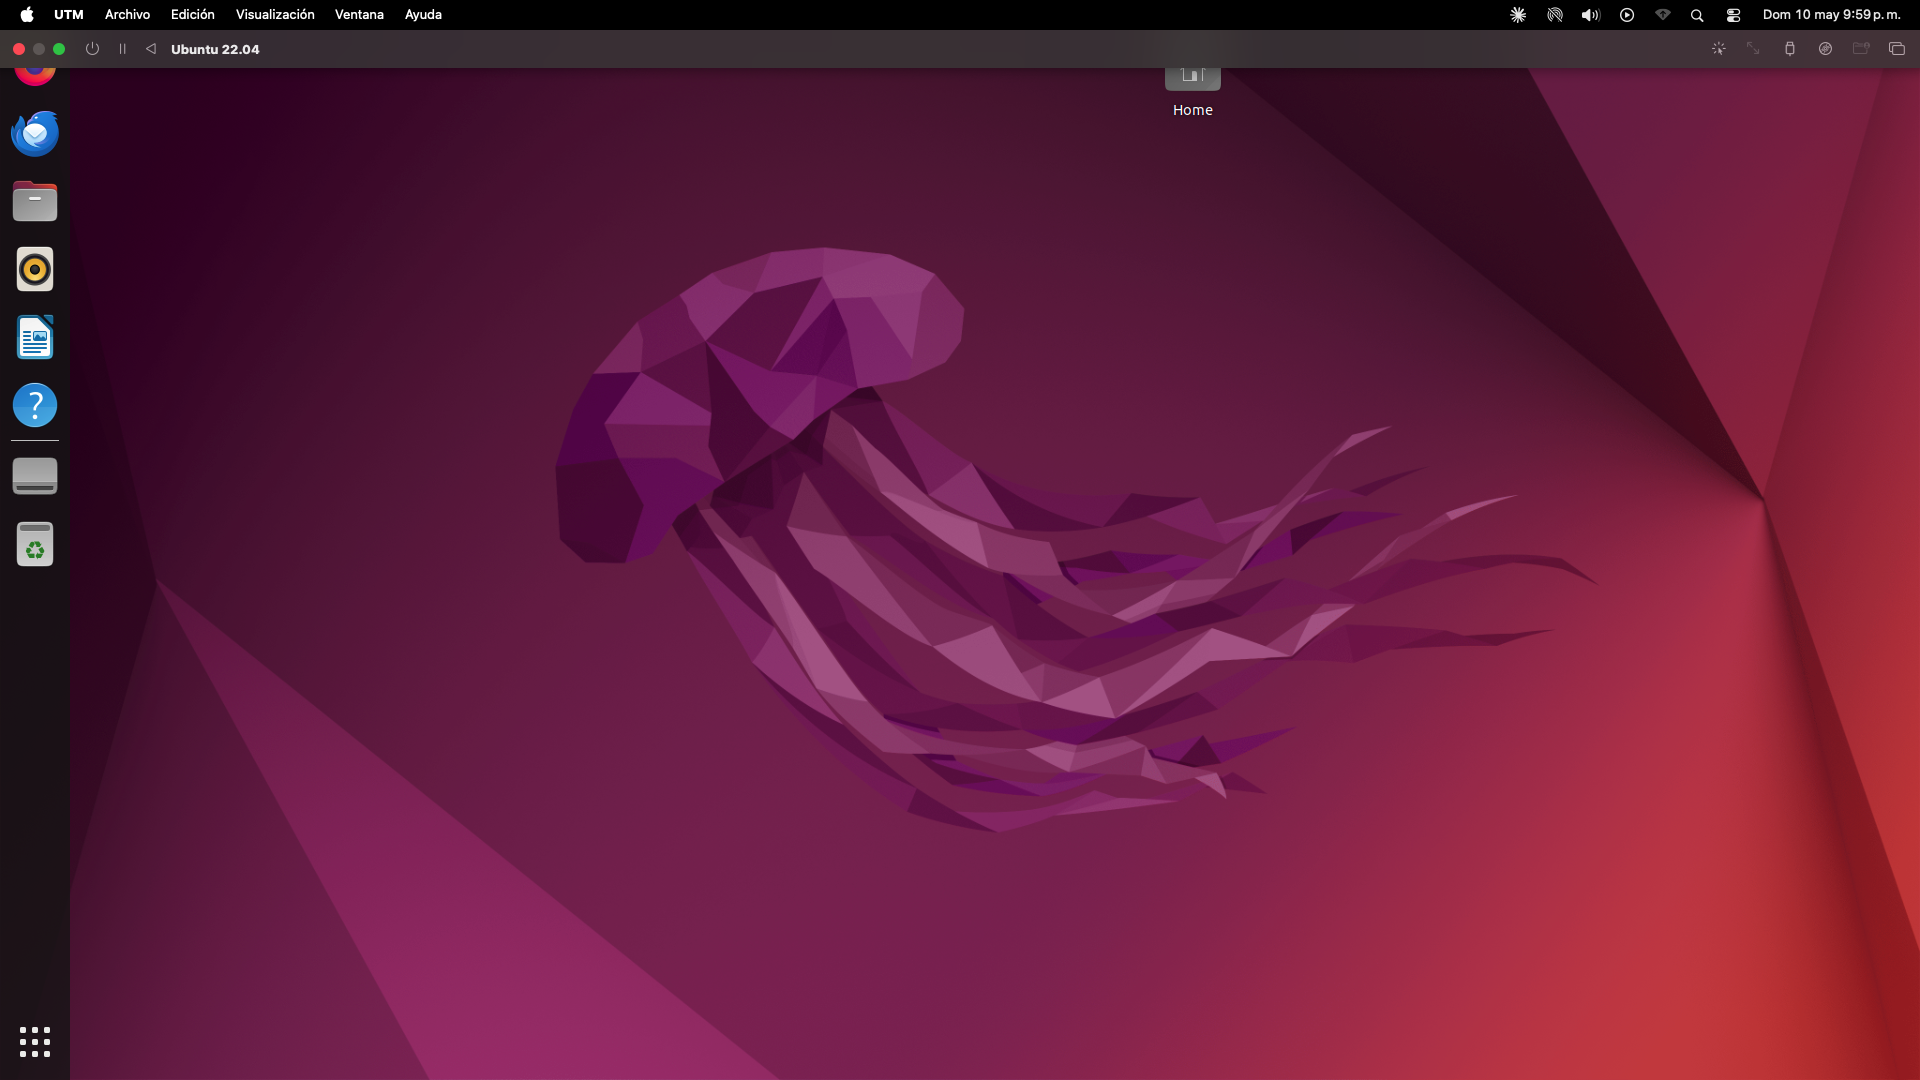
\includegraphics[width=0.85\textwidth]{../../img/environment/ubuntu.png}
  \caption{\textit{Máquina virtual Ubuntu 22.04 con Juice Shop (víctima) en ejecución.}}
\end{figure}

\begin{figure}[H]
  \centering
  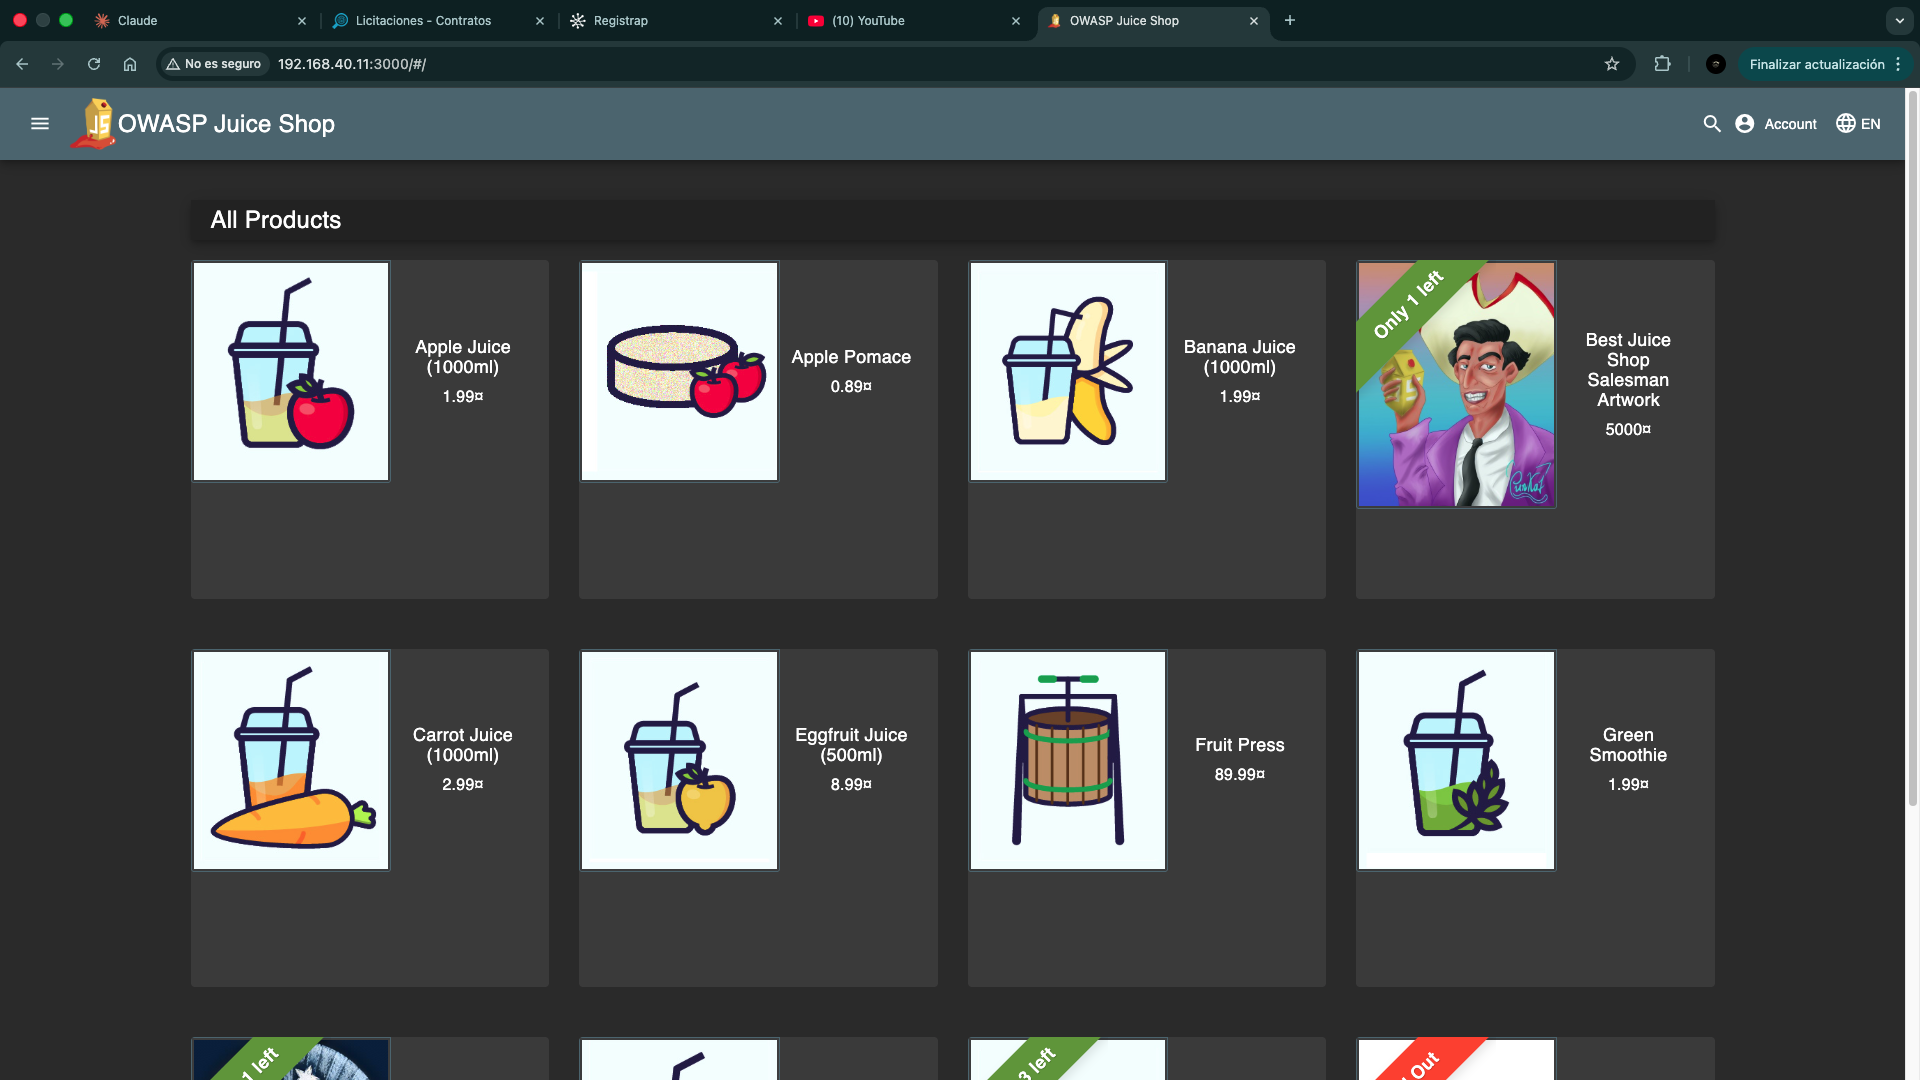
\includegraphics[width=0.85\textwidth]{../../img/juiceshop/juiceShopRunning.png}
  \caption{\textit{OWASP Juice Shop corriendo en el puerto 3000 de la máquina víctima.}}
\end{figure}

% ==========================================================
\section{Tarea 1: SQL Injection --- Bypass de Autenticación}

\subsection{Descripción de la vulnerabilidad}

La inyección SQL (\textit{SQL Injection}) es una vulnerabilidad crítica clasificada bajo \textbf{CWE-89} y la categoría \textbf{A03 -- Inyección} del OWASP Top 10 (2021). Se produce cuando una aplicación web incorpora directamente la entrada del usuario en una consulta SQL sin aplicar sanitización ni usar consultas parametrizadas (\textit{prepared statements}), permitiendo al atacante manipular la lógica de la consulta de base de datos.

En el caso particular del formulario de login de Juice Shop, la consulta SQL que valida las credenciales se construye mediante concatenación directa de los valores ingresados:

\begin{lstlisting}[language=SQL, caption={Consulta SQL vulnerable (simplificada)}]
SELECT * FROM Users WHERE email = '<INPUT_EMAIL>' AND password = '<HASH>'
\end{lstlisting}

Al inyectar el payload \texttt{' OR 1=1--} como valor del campo email, la condición \texttt{WHERE} se transforma en una tautología (siempre verdadera), y los caracteres \texttt{--} comentan el resto de la consulta, eliminando la verificación de contraseña:

\begin{lstlisting}[language=SQL, caption={Consulta SQL resultante tras la inyección del payload}]
SELECT * FROM Users WHERE email = '' OR 1=1--' AND password = '<HASH>'
\end{lstlisting}

La base de datos retorna el primer registro de la tabla \texttt{Users}, que corresponde al administrador (\texttt{admin@juice-sh.op}), autenticando al atacante con privilegios máximos sin conocer ninguna contraseña válida.

\subsection{Herramientas utilizadas}

\begin{itemize}
  \item \textbf{Firefox (Kali Linux)}: Navegador web utilizado para interactuar con el formulario de login de Juice Shop e inyectar el payload directamente en el campo de email.
  \item \textbf{Burp Suite Community Edition}: Proxy HTTP utilizado para interceptar y analizar la petición POST generada al enviar el formulario, permitiendo visualizar el payload en tránsito y confirmar la estructura de la solicitud.
\end{itemize}

\subsection{Pasos realizados}

\subsubsection{Acceso al formulario de login}

Desde el navegador Firefox en la máquina Kali Linux, se navegó a la página de autenticación de Juice Shop:

\begin{lstlisting}[language=bash, caption={URL del formulario de login de Juice Shop}]
http://192.168.40.11:3000/#/login
\end{lstlisting}

\begin{figure}[H]
  \centering
  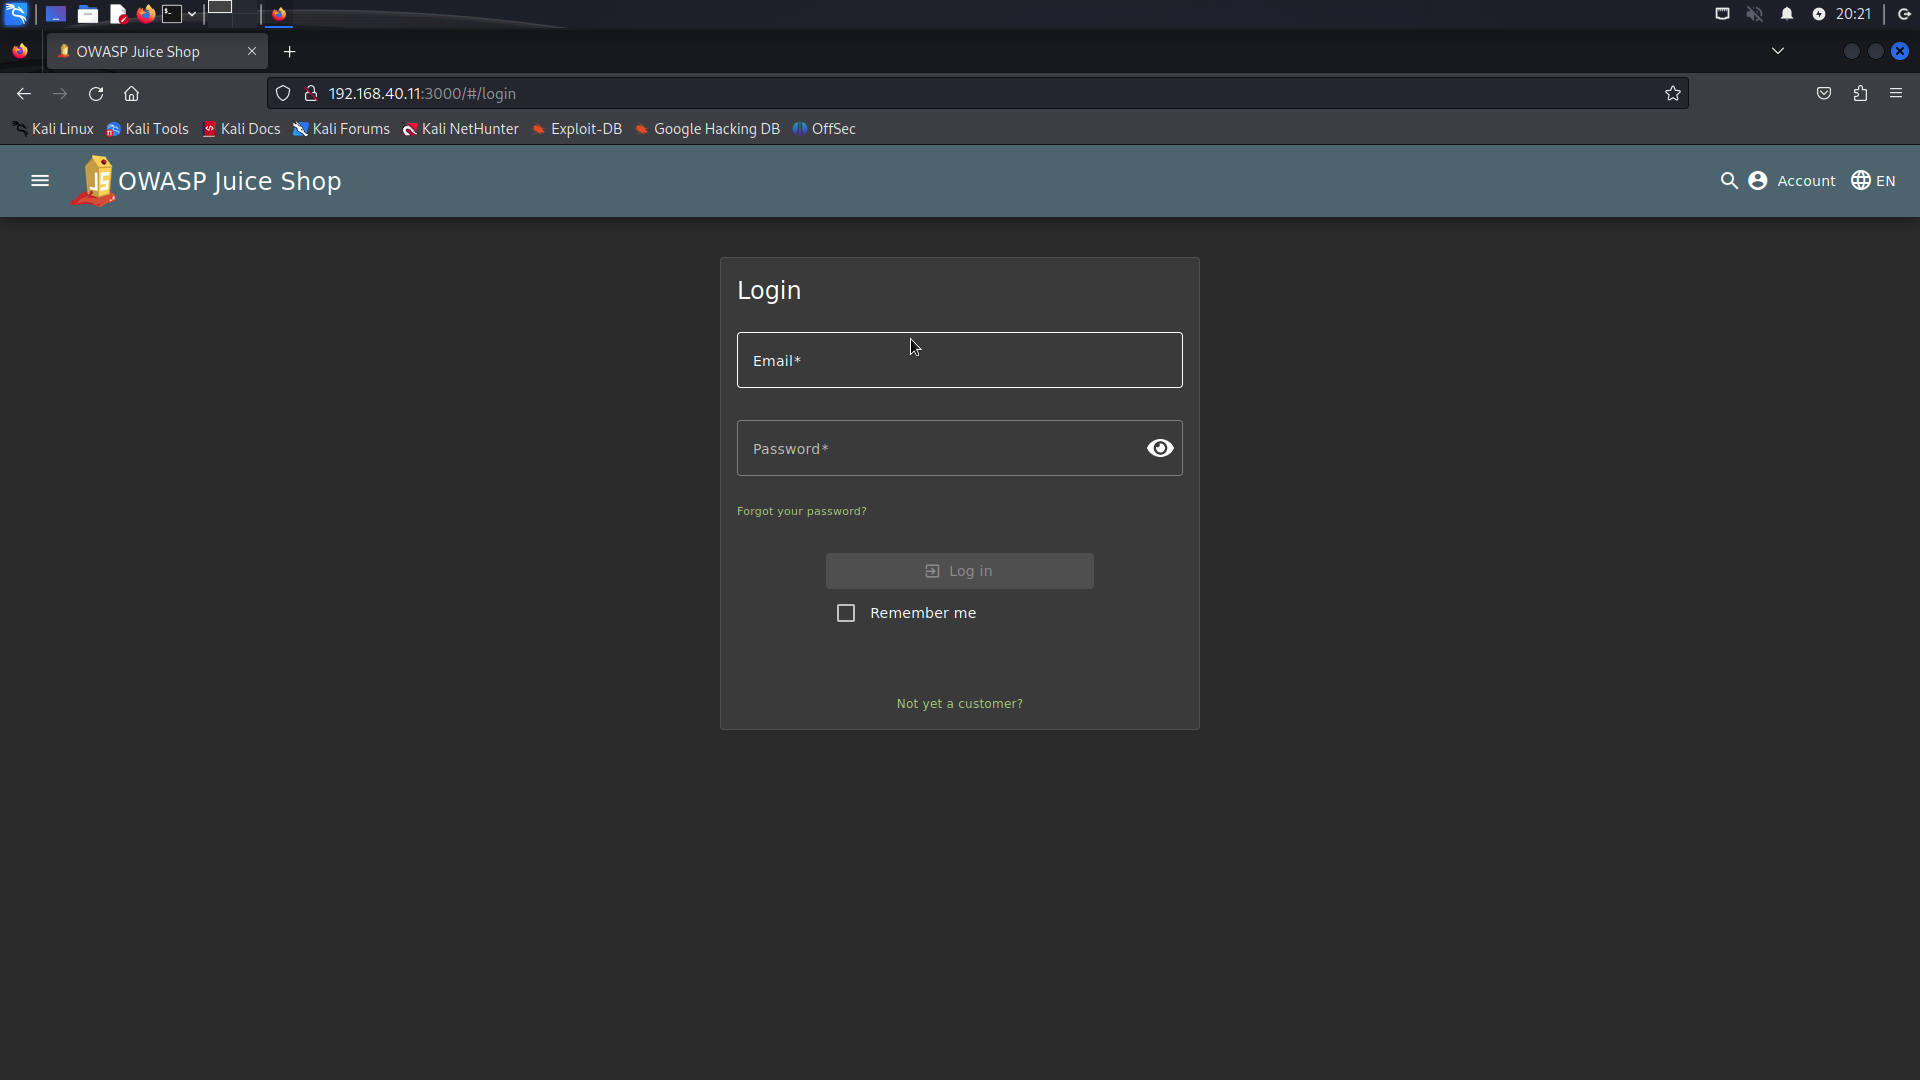
\includegraphics[width=0.92\textwidth]{../../img/tarea1/loginEnkali.png}
  \caption{\textit{Página de login de OWASP Juice Shop accedida desde Firefox en Kali Linux.}}
\end{figure}

\subsubsection{Configuración de Burp Suite como proxy HTTP}

Se configuró Burp Suite Community Edition como proxy HTTP local en el puerto 8080. En Firefox se habilitó la configuración de proxy manual apuntando a \texttt{127.0.0.1:8080}, permitiendo que Burp Suite intercepte todo el tráfico HTTP generado por el navegador. Se activó la opción \textbf{Intercept ON} en la pestaña Proxy de Burp Suite.

\begin{figure}[H]
  \centering
  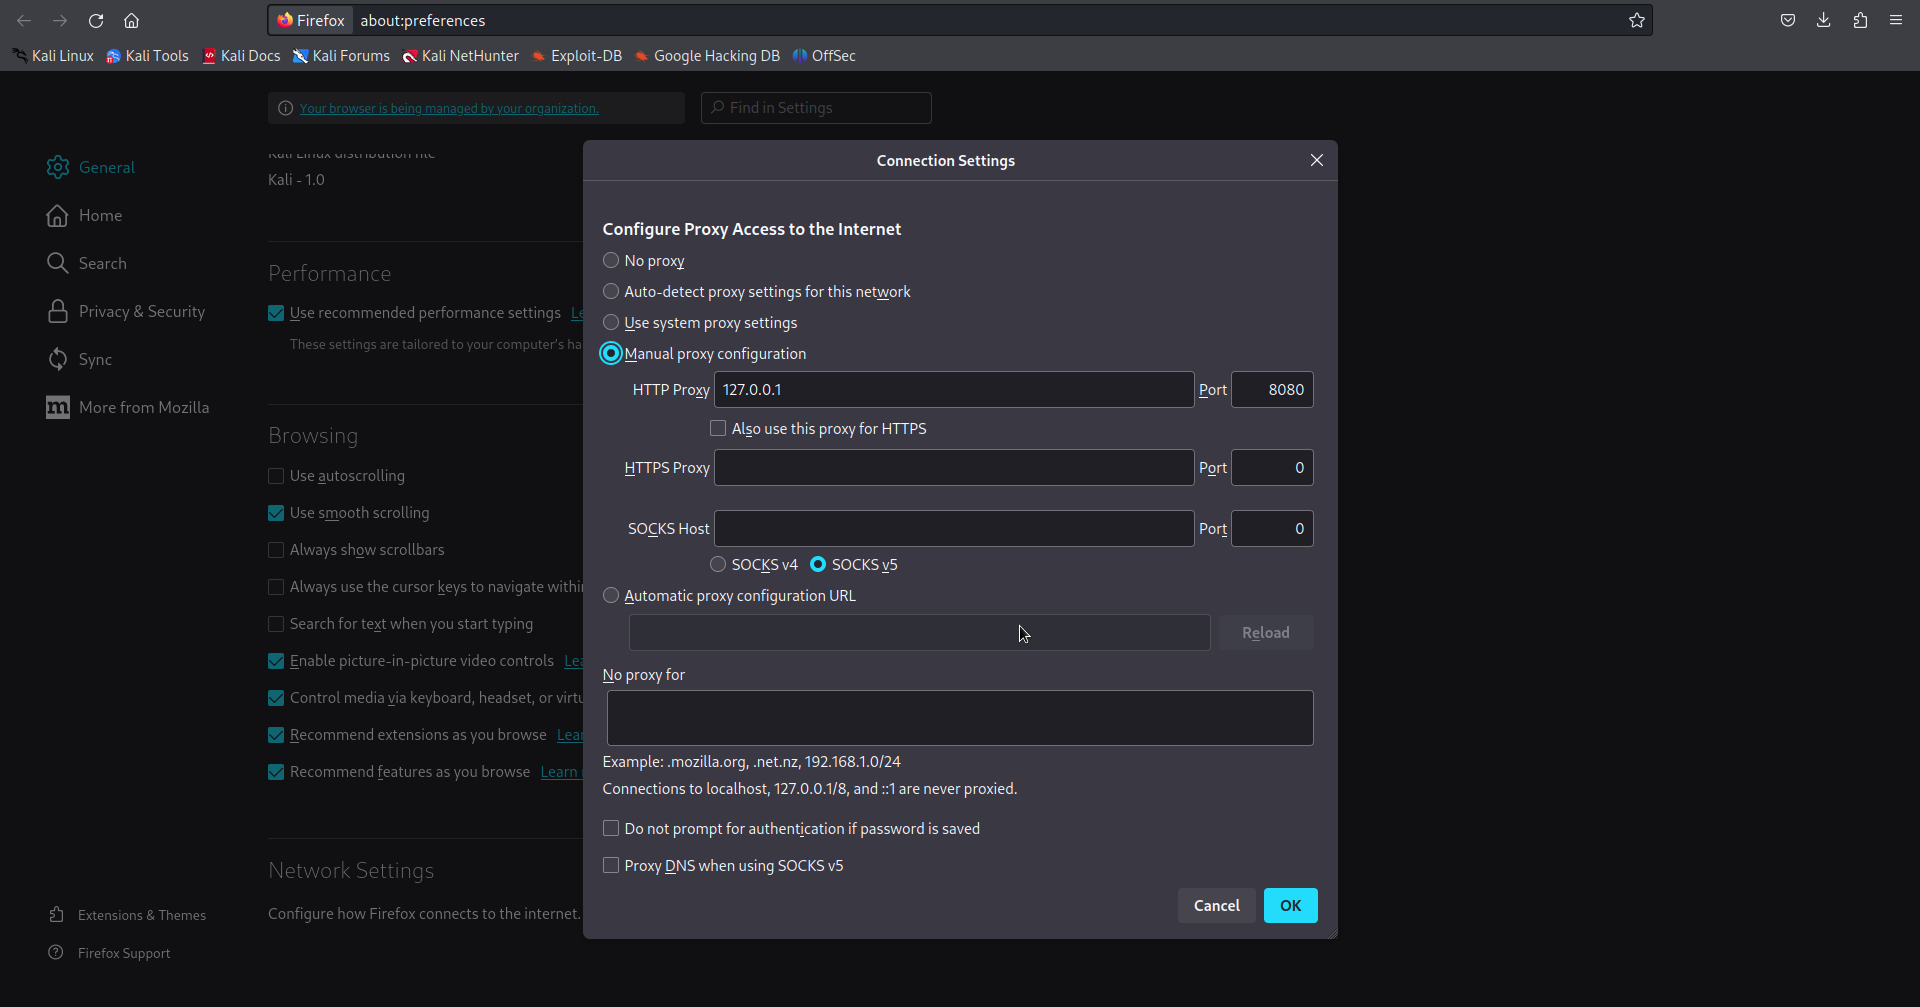
\includegraphics[width=0.92\textwidth]{../../img/tarea1/proxyConfig.png}
  \caption{\textit{Configuración del proxy manual en Firefox apuntando a Burp Suite en 127.0.0.1:8080.}}
\end{figure}

\subsubsection{Inyección del payload}

En el campo \textbf{Email} del formulario se ingresó el siguiente payload:

\begin{lstlisting}[caption={Payload de SQL Injection para bypass de autenticación}]
' OR 1=1--
\end{lstlisting}

En el campo \textbf{Password} se ingresó el valor arbitrario \texttt{a}. La figura siguiente muestra el formulario con el payload listo para enviar.

\begin{figure}[H]
  \centering
  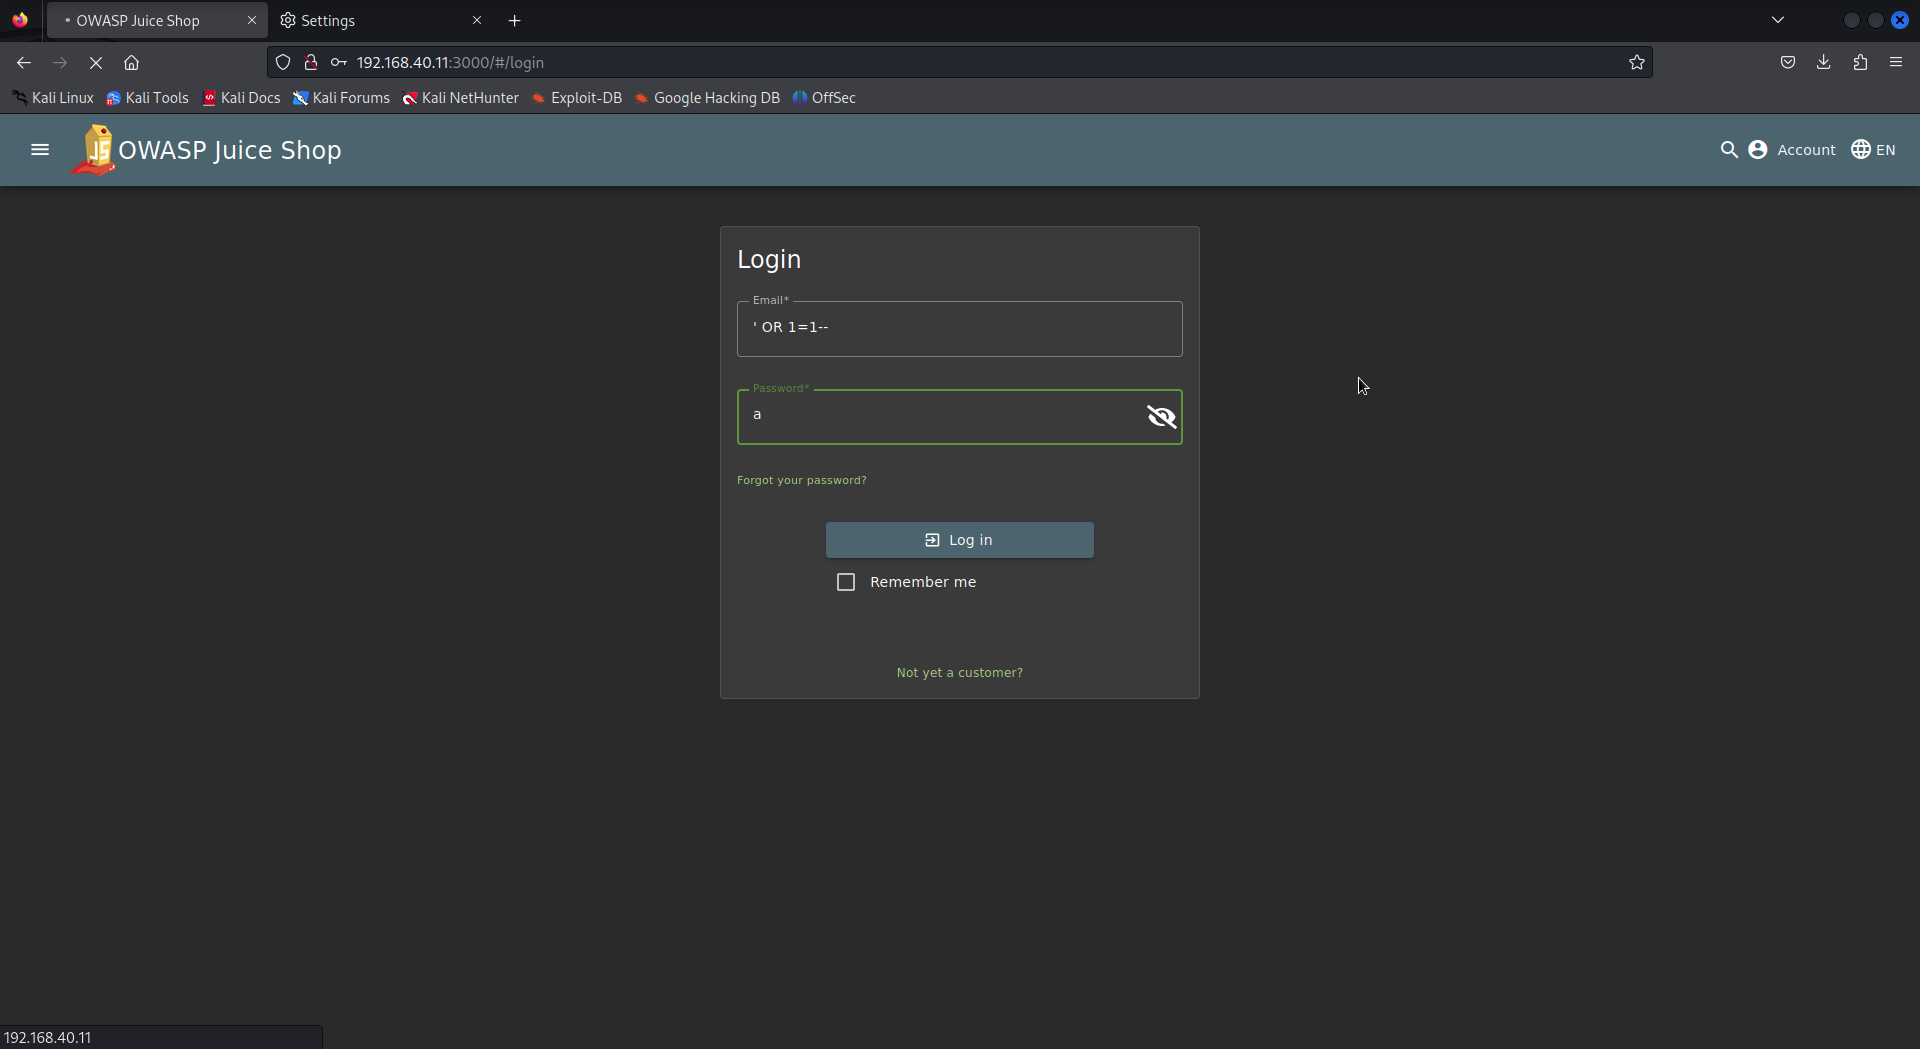
\includegraphics[width=0.92\textwidth]{../../img/tarea1/loginCredentials.png}
  \caption{\textit{Formulario de login de Juice Shop con el payload \texttt{' OR 1=1--} ingresado en el campo Email y valor arbitrario en Password.}}
\end{figure}

\subsubsection{Intercepción de la petición POST en Burp Suite}

Al hacer clic en \textbf{Log in}, Burp Suite interceptó la petición \texttt{POST /rest/user/login} antes de que llegara al servidor. En la vista del \textit{HTTP history} se observa la petición con el método POST, confirmando que el payload fue enviado en el cuerpo de la solicitud hacia el endpoint de autenticación de la API REST de Juice Shop.

\begin{figure}[H]
  \centering
  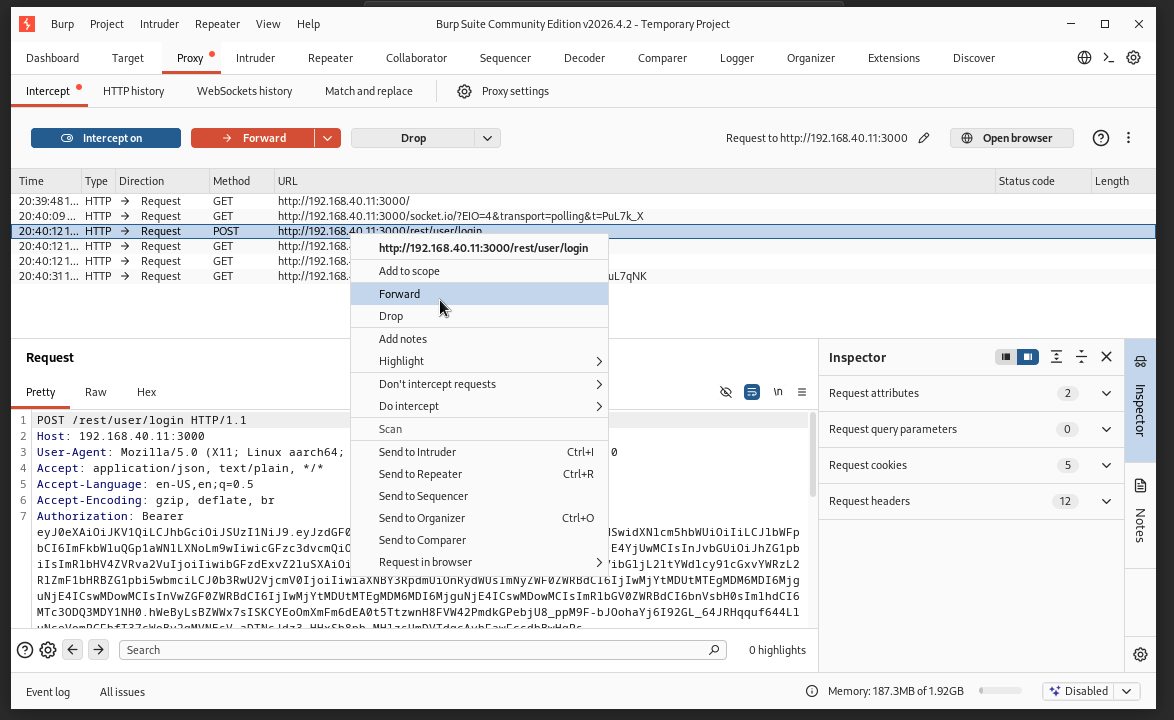
\includegraphics[width=0.92\textwidth]{../../img/tarea1/burpsuite.png}
  \caption{\textit{Petición POST a \texttt{/rest/user/login} interceptada en Burp Suite con el payload de SQL Injection en el cuerpo de la solicitud.}}
\end{figure}

\subsubsection{Verificación del acceso como administrador}

Tras reenviar la petición (\textit{Forward}), Juice Shop procesó la consulta SQL manipulada y autenticó al usuario. La aplicación mostró el banner verde de confirmación del desafío: \textit{``You successfully solved a challenge: Login Admin (Log in with the administrator's user account.)''}, evidenciando el éxito del ataque.

\begin{figure}[H]
  \centering
  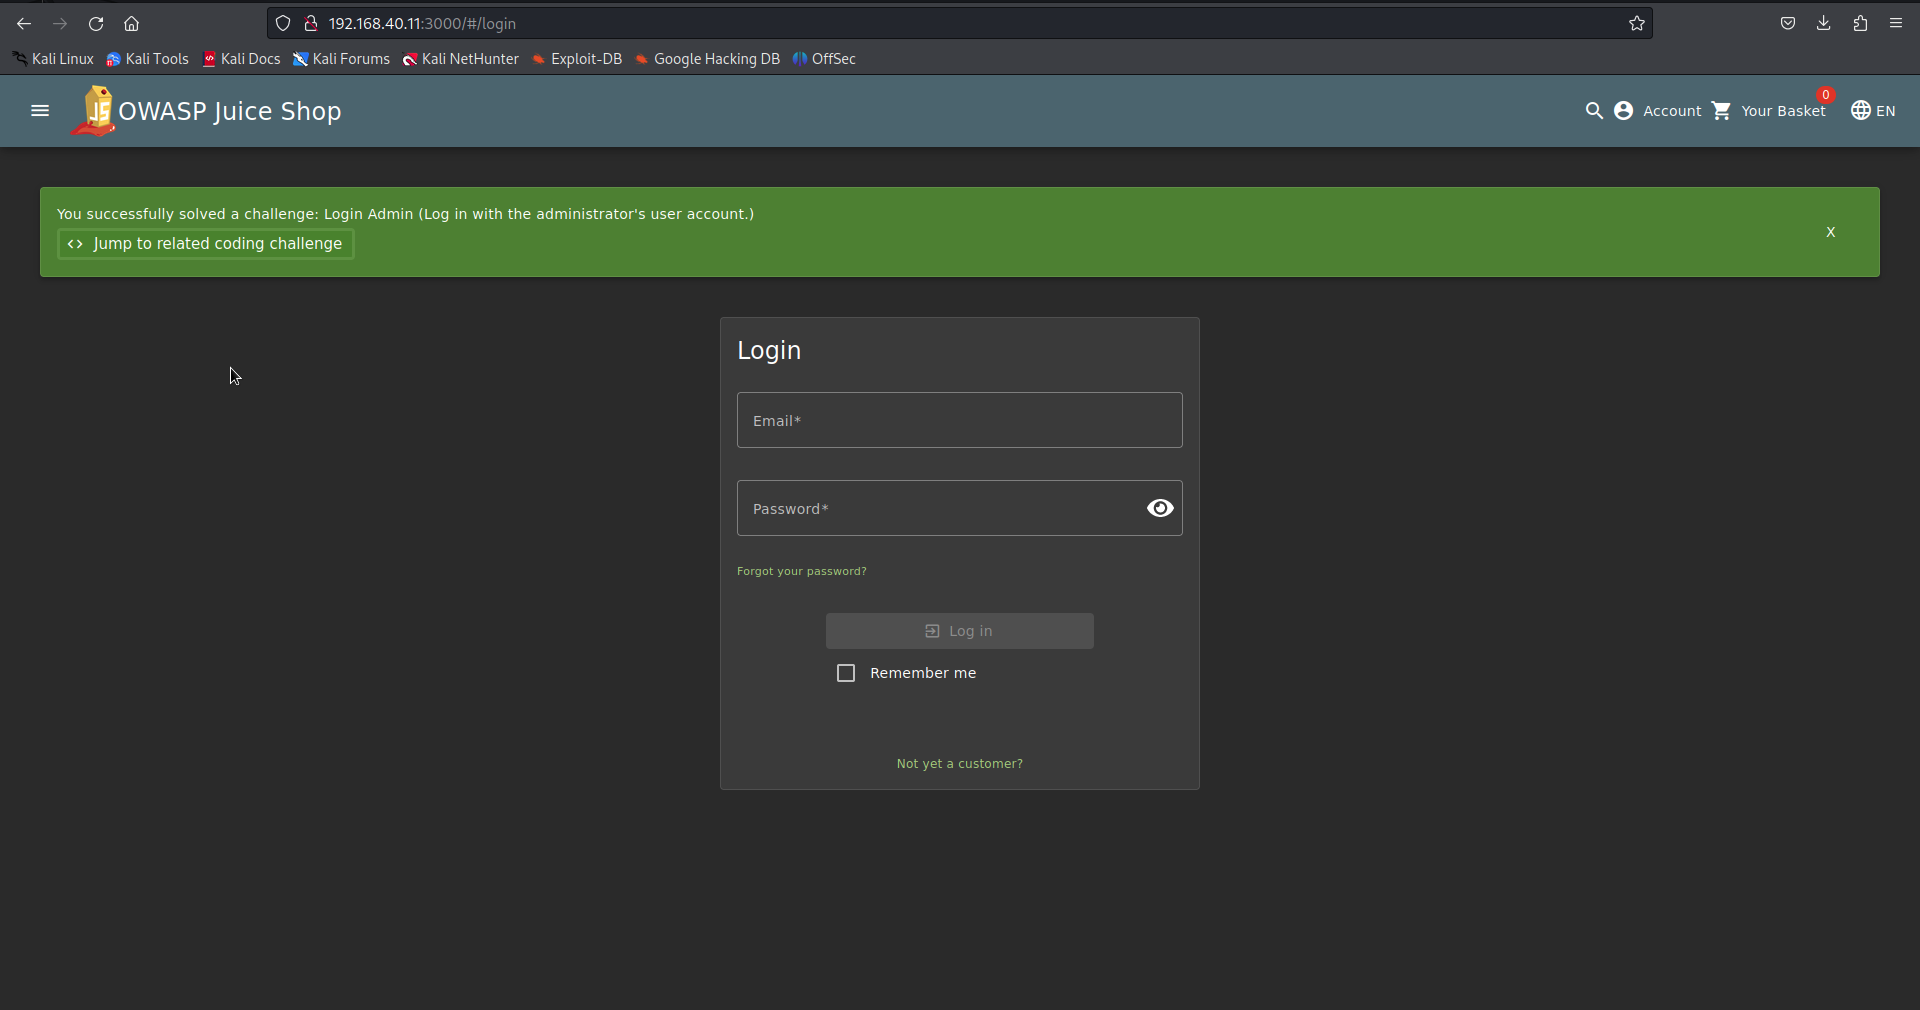
\includegraphics[width=0.92\textwidth]{../../img/tarea1/juiceShopSucess.png}
  \caption{\textit{Banner de confirmación de Juice Shop indicando que el desafío ``Login Admin'' fue resuelto exitosamente mediante SQL Injection.}}
\end{figure}

\begin{figure}[H]
  \centering
  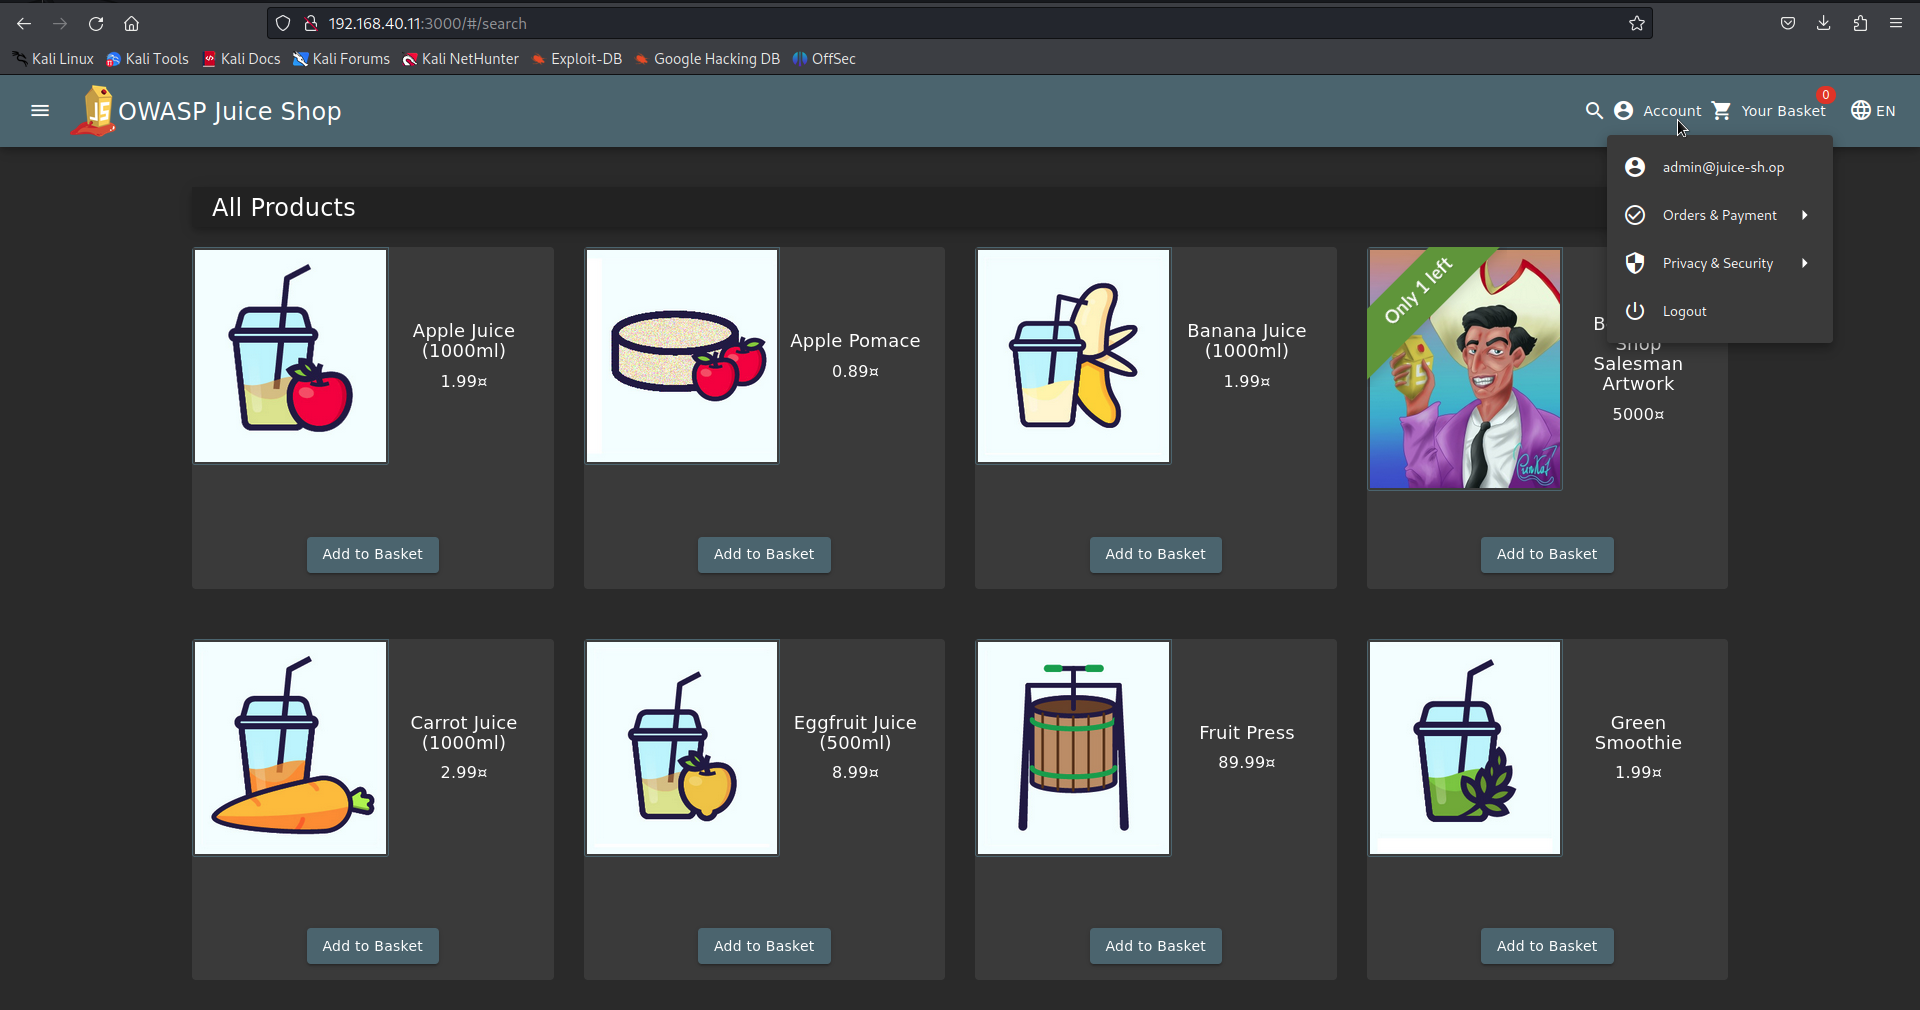
\includegraphics[width=0.92\textwidth]{../../img/tarea1/adminDashboard.png}
  \caption{\textit{Pantalla principal de Juice Shop tras el bypass exitoso, con sesión activa como administrador.}}
\end{figure}

\subsection{Funcionamiento del ataque}

El ataque de SQL Injection para bypass de autenticación sigue el siguiente flujo:

\begin{enumerate}
  \item \textbf{Identificación del punto de inyección}: El formulario de login acepta los campos \texttt{email} y \texttt{password}, que son incorporados sin sanitización en la consulta SQL de verificación de credenciales.
  \item \textbf{Construcción del payload}: El atacante ingresa \texttt{' OR 1=1--} como valor del email. La comilla simple (\texttt{'}) cierra prematuramente el literal de cadena iniciado por la aplicación. La expresión \texttt{OR 1=1} convierte la condición \texttt{WHERE} en una tautología. Los guiones dobles (\texttt{--}) inician un comentario SQL que descarta el resto de la consulta original, incluyendo la verificación de contraseña.
  \item \textbf{Ejecución de la consulta manipulada}: La base de datos SQLite evalúa la condición \texttt{WHERE email = '' OR 1=1}, que es siempre verdadera para cualquier fila. Retorna el primer usuario registrado en la tabla, que es el administrador.
  \item \textbf{Autenticación como administrador}: La aplicación, al recibir un registro de usuario válido, establece una sesión autenticada con los privilegios del usuario retornado (\texttt{admin@juice-sh.op}).
\end{enumerate}

\subsection{Resultado}

Se logró el inicio de sesión exitoso como administrador (\texttt{admin@juice-sh.op}) en OWASP Juice Shop sin conocer ni proporcionar ninguna contraseña válida. El ataque explotó la ausencia de consultas parametrizadas en el módulo de autenticación, demostrando el impacto crítico de la vulnerabilidad CWE-89 (A03 -- Inyección). Un atacante real podría aprovechar este acceso para gestionar usuarios, acceder a órdenes de compra, modificar precios, y obtener información confidencial de todos los clientes registrados en la plataforma.

% ==========================================================
\section{Tarea 2: Sensitive Data Exposure --- Directorio /ftp Expuesto}

\subsection{Descripción de la vulnerabilidad}

La exposición de datos sensibles (\textit{Sensitive Data Exposure}) corresponde a la categoría \textbf{A02 -- Fallos Criptográficos} del OWASP Top 10 (2021) y está catalogada bajo \textbf{CWE-538} (\textit{File and Directory Information Exposure}). Esta vulnerabilidad se produce cuando una aplicación expone recursos o rutas del servidor sin ningún mecanismo de control de acceso ni autenticación, permitiendo a cualquier usuario o atacante acceder a archivos potencialmente confidenciales simplemente conociendo la URL.

En el caso de OWASP Juice Shop, el directorio \texttt{/ftp} del servidor se encuentra completamente accesible desde el navegador sin requerir sesión activa ni credenciales. Este directorio contiene archivos sensibles del negocio, entre ellos planes de adquisición corporativa (\texttt{acquisitions.md}), archivos de configuración cifrados (\texttt{announcement\_encrypted.md}), bases de datos de gestión de incidentes (\texttt{incident-support.kdbx}) y copias de seguridad de dependencias (\texttt{package.json.bak}).

La aplicación intenta restringir parcialmente el acceso a archivos con extensiones consideradas peligrosas (como \texttt{.bak}) retornando un código HTTP 403, pero esta medida es insuficiente: el directorio sigue siendo listable, los archivos con extensión \texttt{.md} se descargan libremente, y la mera existencia de los archivos restringidos queda expuesta en el listado.

\subsection{Herramientas utilizadas}

\begin{itemize}
  \item \textbf{Firefox (Kali Linux)}: Navegador web utilizado para acceder y visualizar el listado del directorio \texttt{/ftp} sin autenticación.
  \item \textbf{curl}: Herramienta de transferencia de datos por línea de comandos utilizada para descargar archivos individuales del directorio expuesto y examinar las cabeceras HTTP de respuesta del servidor.
\end{itemize}

\subsection{Pasos realizados}

\subsubsection{Acceso al directorio /ftp sin autenticación}

Sin haber iniciado sesión en la aplicación, se navegó directamente al directorio \texttt{/ftp} desde Firefox en Kali Linux:

\begin{lstlisting}[language=bash, caption={URL del directorio FTP expuesto}]
http://192.168.40.11:3000/ftp
\end{lstlisting}

El servidor respondió mostrando un listado completo de archivos sin solicitar credenciales. El directorio contenía los siguientes archivos: \texttt{acquisitions.md}, \texttt{announcement\_encrypted.md}, \texttt{coupons\_2013.md.bak}, \texttt{eastere.gg}, \texttt{encrypt.pyc}, \texttt{incident-support.kdbx}, \texttt{legal.md}, \texttt{package-lock.json.bak}, \texttt{package.json.bak} y \texttt{suspicious\_errors.yml}, además de una carpeta \texttt{quarantine/}.

\begin{figure}[H]
  \centering
  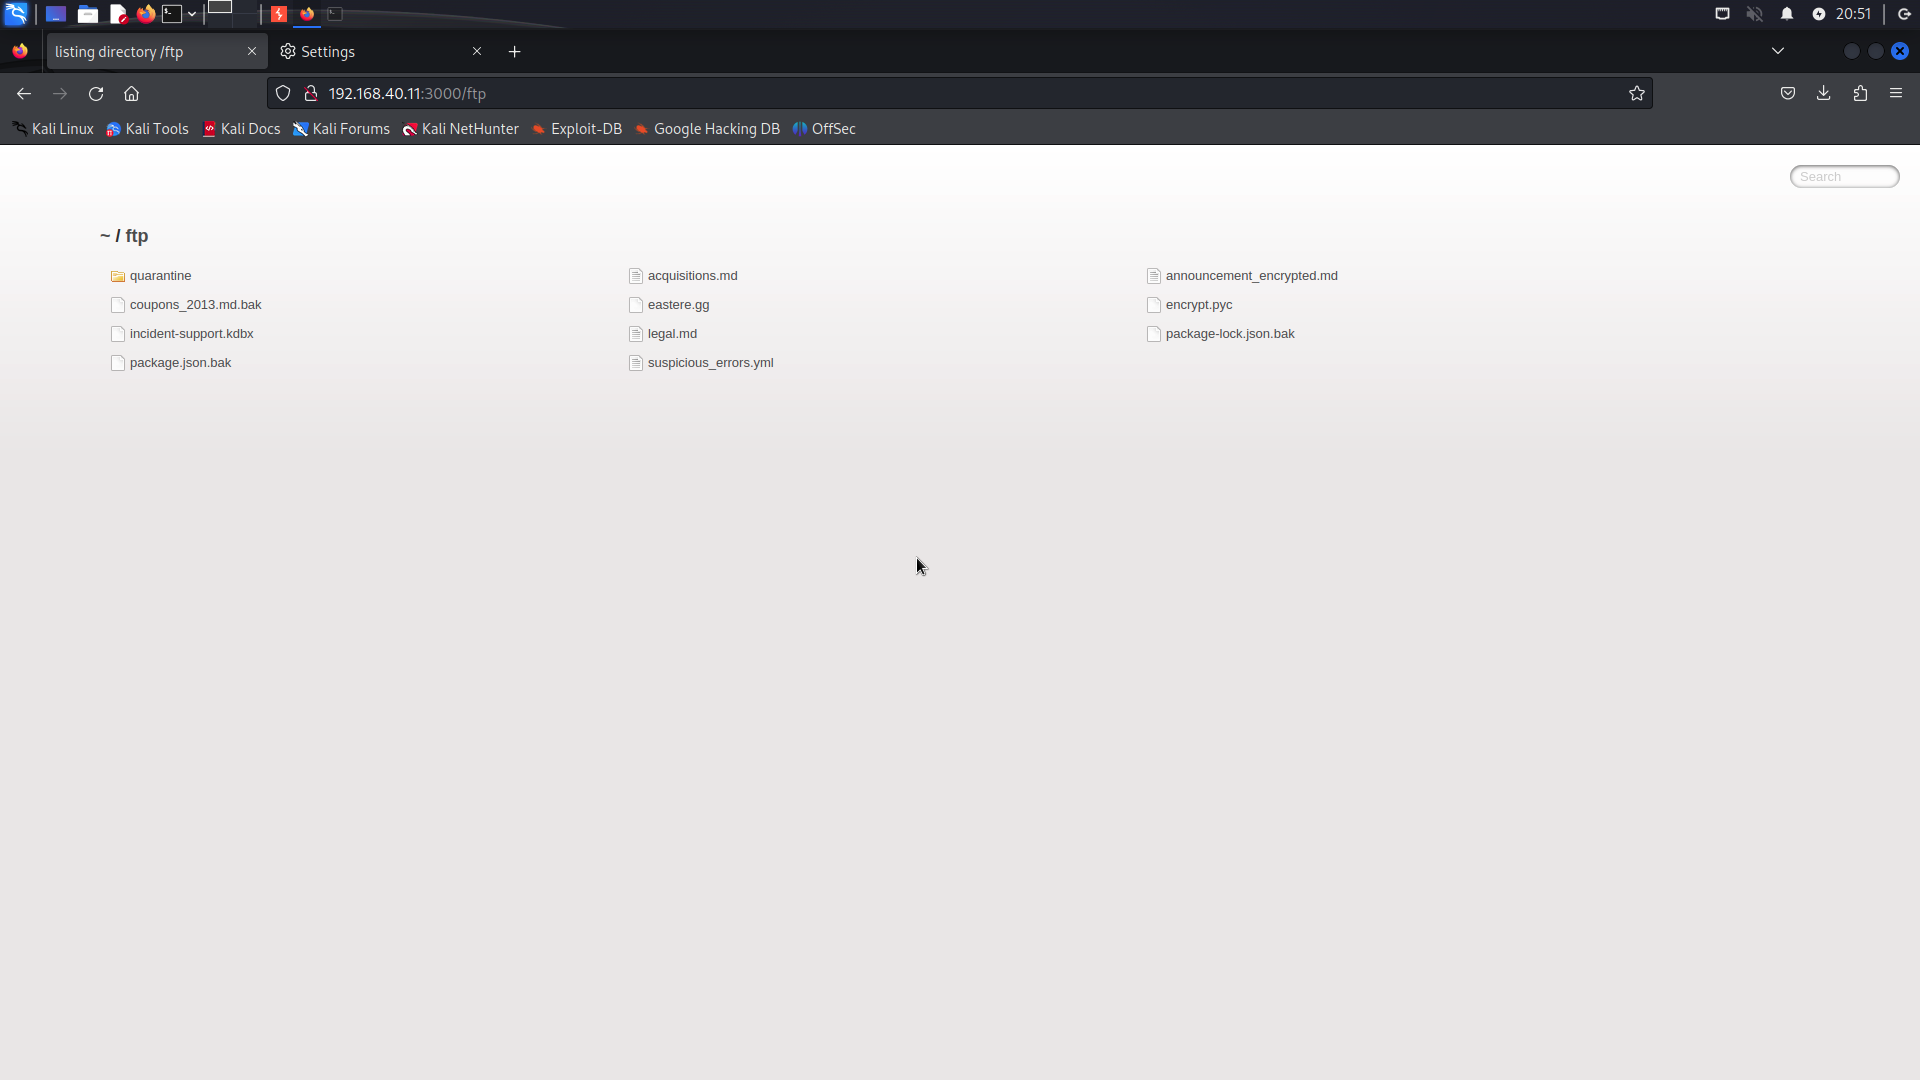
\includegraphics[width=0.92\textwidth]{../../img/tarea2/t2_ftp_directory.png}
  \caption{\textit{Listado del directorio \texttt{/ftp} de Juice Shop accedido desde Firefox en Kali Linux sin ningún tipo de autenticación.}}
\end{figure}

\subsubsection{Descarga de acquisitions.md con curl}

Desde la terminal de Kali Linux se utilizó \texttt{curl} con la opción \texttt{-v} (verbose) para descargar el archivo \texttt{acquisitions.md} y examinar las cabeceras de la respuesta HTTP:

\begin{lstlisting}[language=bash, caption={Descarga del archivo de adquisiciones mediante curl}]
mkdir -p ~/tarea2
cd ~/tarea2
curl -v http://192.168.40.11:3000/ftp/acquisitions.md -o acquisitions.md
echo "--- CONTENIDO DEL ARCHIVO ---"
cat acquisitions.md
\end{lstlisting}

El servidor respondió con código \textbf{HTTP 200 OK}, transfiriendo 909 bytes con tipo de contenido \texttt{text/markdown}. El archivo reveló información corporativa altamente sensible: planes de adquisición de competidores con impacto en el mercado bursátil, marcados explícitamente como \textit{``This document is confidential! Do not distribute!''}.

\begin{figure}[H]
  \centering
  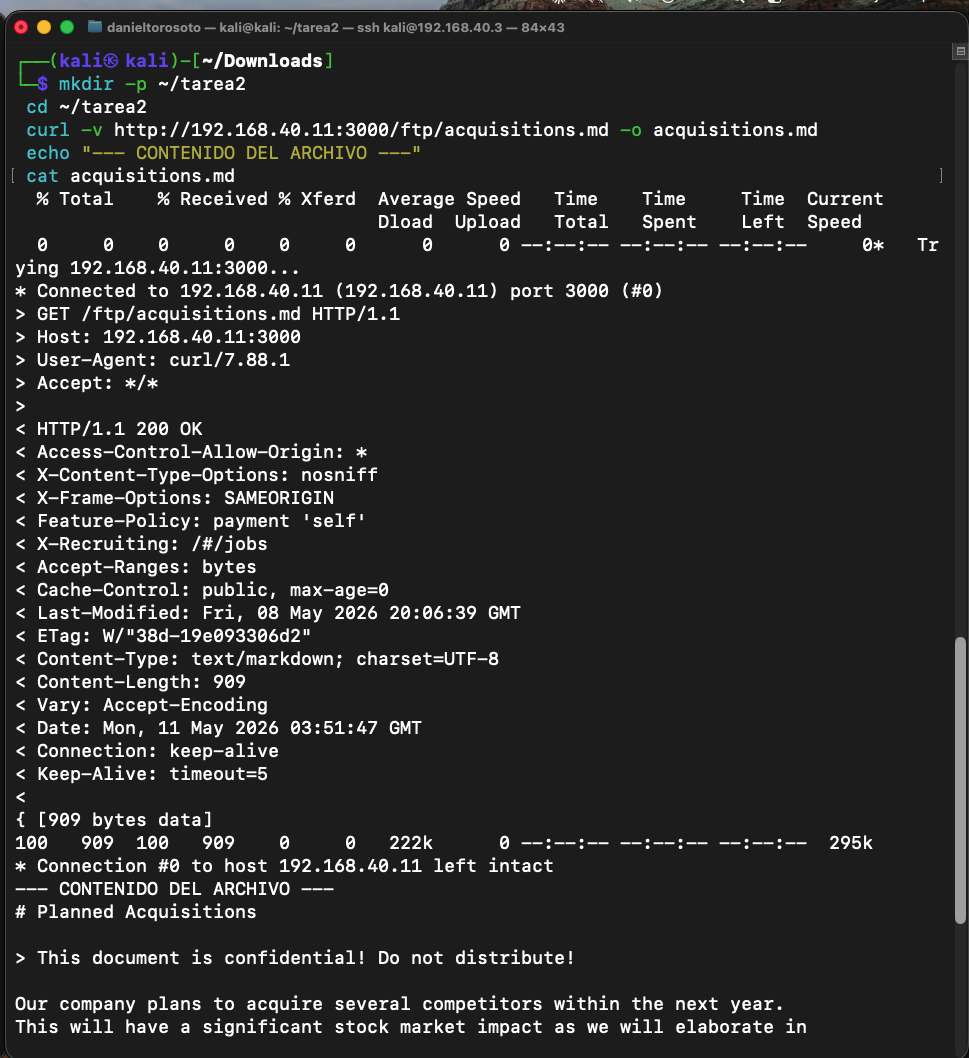
\includegraphics[width=0.92\textwidth]{../../img/tarea2/t2_acquisitions_download.png}
  \caption{\textit{Descarga exitosa de \texttt{acquisitions.md} mediante curl (HTTP 200 OK) y visualización de su contenido confidencial en la terminal de Kali Linux.}}
\end{figure}

\subsubsection{Intento de descarga de package.json.bak}

Se intentó descargar el archivo \texttt{package.json.bak}, que podría revelar las dependencias exactas y versiones del proyecto, útiles para identificar vulnerabilidades conocidas en las bibliotecas utilizadas:

\begin{lstlisting}[language=bash, caption={Intento de descarga de package.json.bak}]
curl -v http://192.168.40.11:3000/ftp/package.json.bak -o package.json.bak
head -20 package.json.bak
\end{lstlisting}

El servidor respondió con \textbf{HTTP 403 Forbidden} y el mensaje \textit{``Error: Only .md and .pdf files are allowed!''}, denegando el acceso a archivos con extensión \texttt{.bak}. Sin embargo, esta restricción resulta insuficiente como medida de seguridad: el archivo es visible en el listado del directorio, confirmando su existencia, y la restricción solo aplica a ciertas extensiones, dejando accesibles otros archivos sensibles como \texttt{.md} o \texttt{.pyc}.

\begin{figure}[H]
  \centering
  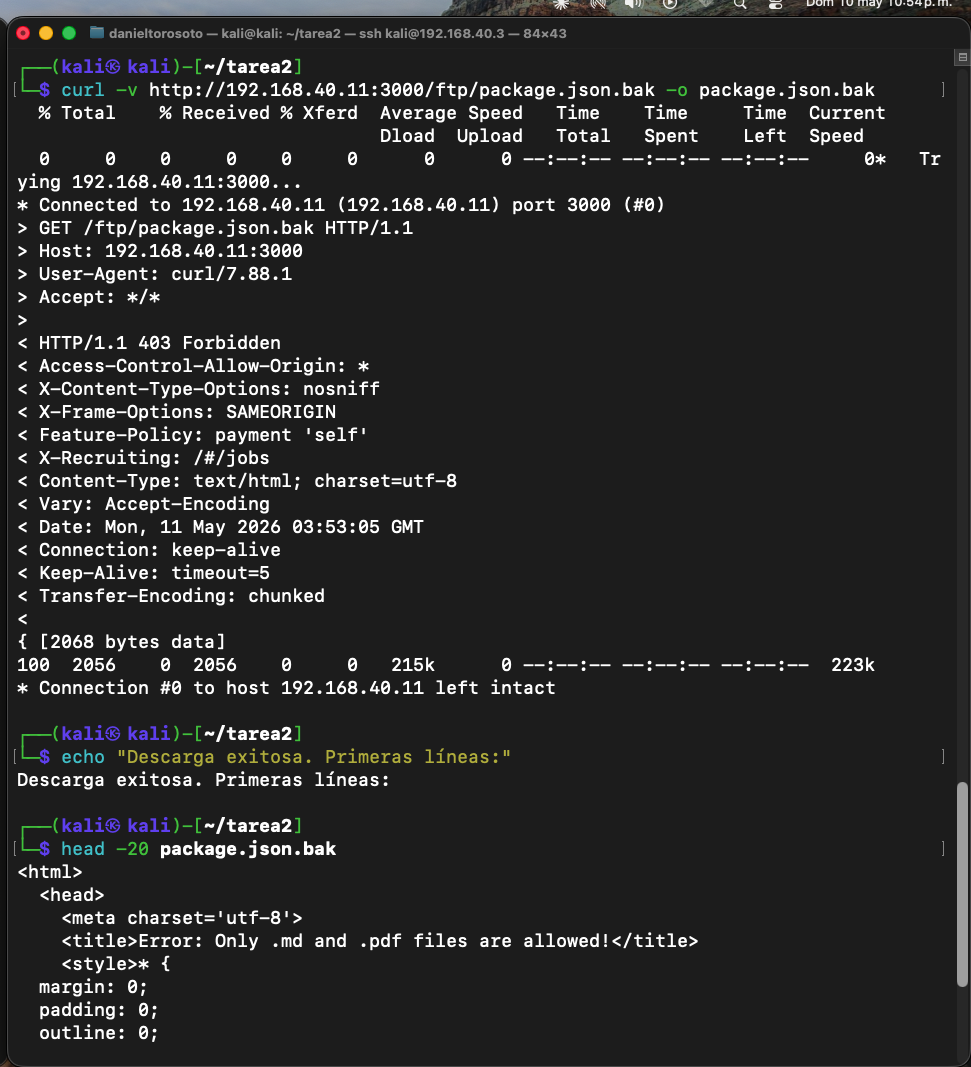
\includegraphics[width=0.92\textwidth]{../../img/tarea2/t2_curl_output.png}
  \caption{\textit{Respuesta HTTP 403 Forbidden al intentar descargar \texttt{package.json.bak}. El mensaje de error expone la lógica de filtrado del servidor, evidenciando una restricción parcial e insuficiente.}}
\end{figure}

\subsection{Funcionamiento del ataque}

La vulnerabilidad de exposición del directorio \texttt{/ftp} sigue el siguiente flujo de explotación:

\begin{enumerate}
  \item \textbf{Descubrimiento de la ruta}: El atacante, mediante reconocimiento web (herramientas de fuzzing de directorios como \texttt{gobuster} o \texttt{dirbuster}, o simplemente conocimiento previo de la estructura de Juice Shop), identifica la ruta \texttt{/ftp} como accesible públicamente.
  \item \textbf{Listado del directorio}: El servidor Node.js de Juice Shop sirve el directorio sin verificar si el solicitante posee una sesión autenticada. El listado completo de archivos queda expuesto, revelando la existencia de documentos sensibles.
  \item \textbf{Descarga de archivos sin restricción}: Archivos con extensiones \texttt{.md}, \texttt{.pyc}, \texttt{.gg} y \texttt{.yml} se transfieren con código HTTP 200 ante cualquier solicitud GET, sin verificar autenticación, rol o permisos del solicitante.
  \item \textbf{Restricción parcial bypasseable}: La única defensa implementada es un filtro de extensiones que bloquea \texttt{.bak} y similares con HTTP 403. Esta medida es trivialmente insuficiente: no oculta la existencia de los archivos, no protege las extensiones permitidas, y puede ser evadida mediante técnicas de path traversal o manipulación de la solicitud HTTP en versiones vulnerables.
\end{enumerate}

\subsection{Resultado}

Se accedió y descargó exitosamente el archivo \texttt{acquisitions.md} desde el directorio \texttt{/ftp} de Juice Shop sin ningún tipo de autenticación, obteniendo documentación corporativa marcada como confidencial que detalla planes de adquisición de competidores con potencial impacto en el mercado bursátil. Adicionalmente, se verificó la existencia de múltiples archivos de alto valor informativo en el directorio expuesto: bases de datos de gestión de incidentes (\texttt{incident-support.kdbx}), copias de seguridad de configuración (\texttt{package.json.bak}), y código Python compilado (\texttt{encrypt.pyc}). La restricción parcial implementada mediante filtrado de extensiones resultó ser una medida de seguridad por oscuridad, insuficiente para proteger los recursos expuestos. Esta vulnerabilidad corresponde a la categoría \textbf{CWE-538} y \textbf{A02 -- Fallos Criptográficos} del OWASP Top 10 (2021).

% ==========================================================
\section{Tarea 3: Broken Access Control --- API de Usuarios sin Autenticación}

\textit{(Pendiente de documentación)}

% ==========================================================
\end{document}
